% !TeX spellcheck = it_IT
\newpage
\section{Address translation}
Gli obiettivi sono:
\begin{itemize}
	\item \textbf{Protezione} della memoria
	\item \textbf{Condivisione} della memoria
	\item Piazzamento in memoria \textbf{flessibile}
	\item Indirizzi \textbf{sparsi}
	\item \textbf{Ricerca efficiente} a runtime
	\item Tabelle di traduzione \textbf{compatte}
	\item \textbf{Portabilità}
\end{itemize}
\begin{center}
	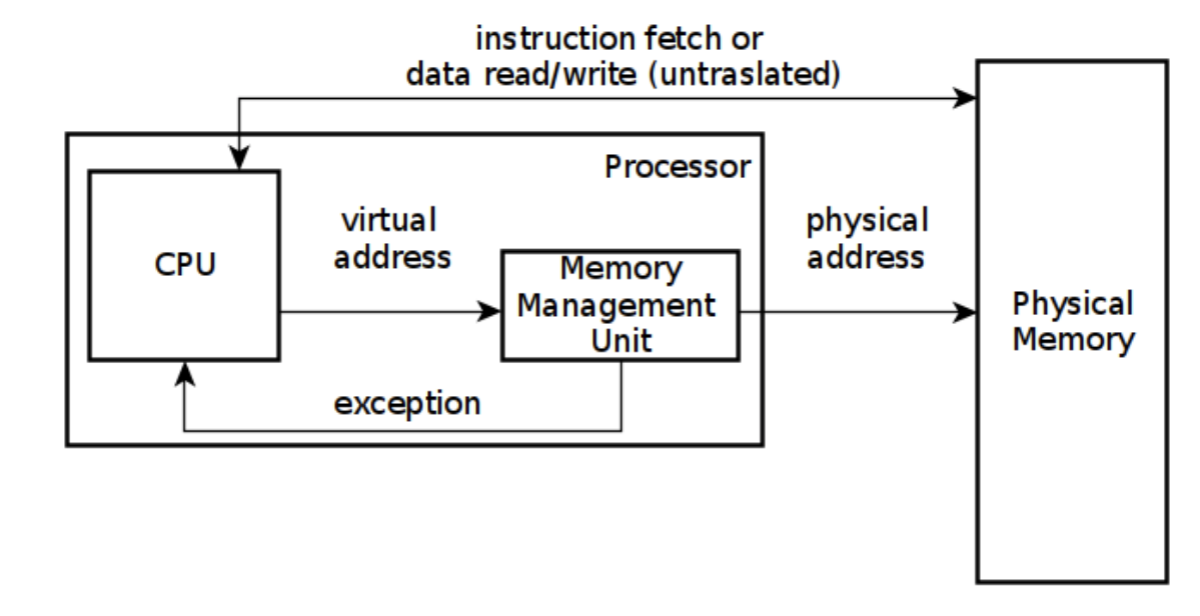
\includegraphics[scale=0.3]{address_translation.png}
\end{center}
\subsection{Virtual base and Bounds}
Ad ogni processo si assegna un \textbf{base register}, ovvero un limite inferiore alla zona di memoria, e un \textbf{bound register}, ovvero un limite superiore.
La \textbf{Memory Management Unit} si occupa di verificare che l'indirizzo richiesto sia nel range che è stato assegnato al programma in esecuzione ed effettua poi la traduzione dell'indirizzo in quello effettivo della memoria fisica.
\begin{center}
	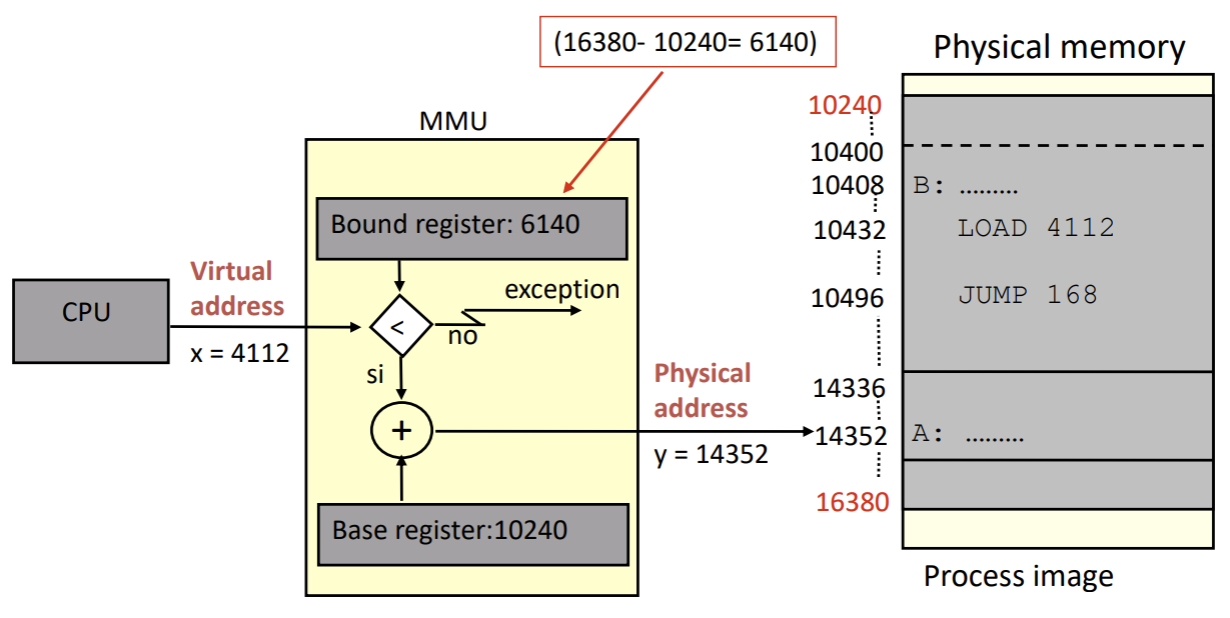
\includegraphics[scale=0.3]{base_bounds.png}
\end{center}
\subsubsection{Variable partitions}
Se la gestione avviene con le partizioni di memoria, questa può diventare \textbf{frammentata}. Bisogna quindi decidere dove allocare ogni volta una nuova partizione.
\begin{center}
	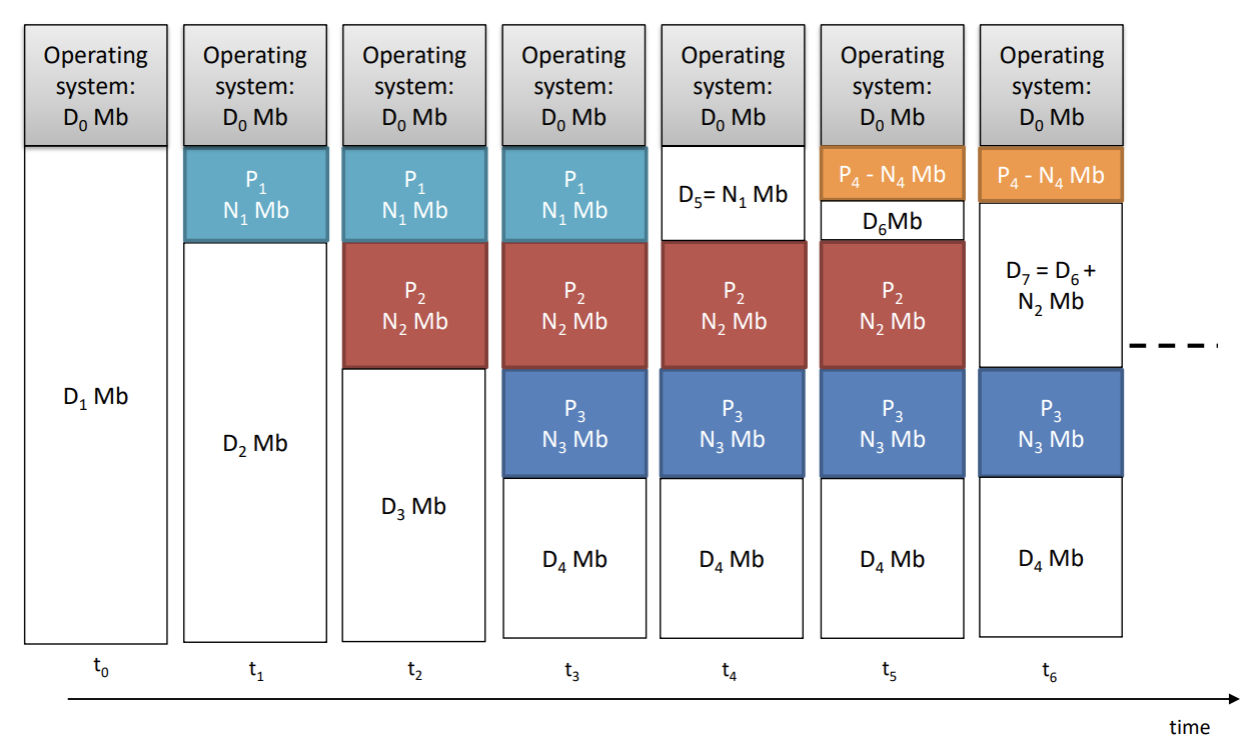
\includegraphics[scale=0.25]{variable_partitions.png}
\end{center}

\subsubsection{Frammentazione}
La frammentazione della memoria può presentarsi in due modi:
\begin{itemize}
	\item \textbf{Interna}: la memoria viene allocata ad una partizione ma non viene usata dal processo. Avviene con le partizioni di dimensione \textbf{fissa}.
	\item \textbf{Esterna}: le partizioni libere di memoria sono troppo piccole per essere usate per altre allocazioni anche se la memoria totale libera sarebbe sufficiente. Si presenta con le partizioni \textbf{variabili}.
\end{itemize}
\begin{definition}[Deframmentazione]
	La deframmentazione della memoria è il processo di spostare le partizioni allocate l'una vicina all'altra in modo da avere lo spazio libero tutto contiguo.
\end{definition}
\subsubsection{Allocazione}
Esistono due tecniche di ottimizzazione per allocare una nuova partizione:
\begin{itemize}
	\item \textbf{First-fit}: tra le partizioni libere, seleziona la \textit{prima} grande a sufficienza
	\item \textbf{Best-fit}: tra le partizioni libere, seleziona la \textit{più piccola} che è grande a sufficienza
\end{itemize}
\subsubsection{Conclusione}
È un metodo \textbf{semplice} e veloce che però non ha \textit{coarse-grain protection}, non permette la condivisione tra processi e non può far crescere a richiesta \textit{stack} e \textit{heap}.

\subsection{Segmentazione}
Un \textbf{segmento}